\chapter{Programmable Realtime Unit}
\label{chap:pru}

This chapter will discuss the capabilities, and usage of the Programmable Realtime Unit (\textls{PRU}).

Even with realtime operating systems, no process can allocate hundred percent time of a CPU. There are essential OS management tasks, which handles the hardware. These management tasks need to be executed periodically.

\section{Example}
\label{subsec:example}

This example illustrates the usability of an external control unit, if the system has rigorous timing criteria.

\begin{figure}[h]
	\centering
	\begin{tikzpicture}[
			squarednode/.style={
				rectangle,
				draw=black,
				very thick,
				minimum height=2cm,
				minimum width=2.5cm,
				inner sep=.2cm,
			},
			label/.style={
				font=\footnotesize
			}
		]
		\node[squarednode] (A) [] {\rtos};
		\node[squarednode] (B) [right = 4cm of A] {Controller};

		\draw[thick,->] (A.east) -- ++(4,0) node[above,pos=0.12] (AB) {};
		\draw[very thick,->] (B.east) -- ++(4,0) node[midway,above,text width = 3cm] {To controlled unit};
		\timing (AB) {6{1C0.5C}C};
	\end{tikzpicture}
	\caption{A bit--banging solution}
	\label{fig:example_pwm}
\end{figure}

\cref{fig:example_pwm} depicts the example. Our example consist of a computer (\rtos), and a controller. The \rtos component is sending a pulse width modulated signal (\pwm) to the controller. The controlling computer does not have an integrated \pwm controller, and the signal modulation must done by software. This method, when a commonly hardware peripheral is emulated called \emph{bit--banging}.

Let's say the controller needs a very precise signal, because a small change in the width of the modulated signal cause a big difference in the output of the controller. This means the solution needs the smallest reachable jitter.

This example relies on the measurements of \citep{rt-sched-thesis}, which uses the same development platform this chapter will discuss. It is important to point out the measurements were done on a soft real--time OS. Other commercial products which specializes in hard real--time (VxWorks, µC/OS-II) might reach better performance, but this chapter will reveal alternate solutions.

\subsubsection{Evaluation}

At PWM frequency 50ms, the system was capable of a completely precision software based control. At 10ms, the best achievable jitter was $1.32\%$, and at 1ms, $4.1\%$.
Because the computer is not totally dedicated to generate our control signal, jitter can happen. If our specification has low jitter requirements, this solution is not applicable to our design.

\section{Delegation of real--time functionality}

One possibile solution for \cref{subsec:example} is to delegate this task to an external coprocessor.

\begin{figure}[h]
	\centering
	\begin{tikzpicture}[
			squarednode/.style={
				rectangle,
				draw=black,
				very thick,
				minimum height=2cm,
				minimum width=2.5cm,
				inner sep=.2cm,
			},
			label/.style={
				font=\footnotesize
			}
		]
		\node[squarednode] (A) [] {\rtos};
		\node[squarednode] (B) [right = 2cm of A] {Microcontroller};
		\node[squarednode] (C) [right = 2cm of B] {Controller};

		\draw[thick,->] (A.east) -- ++(2,0) node[midway, above]{\small Command};
		\draw[thick,->] (B.east) -- ++(2,0) node[above,pos=0.12] (AB) {};
		\draw[very thick,->] (C.east) -- ++(2,0) node[midway,above,text width = 1.8cm] {To controlled unit};
		\timing (AB) {2{1C0.5C}C};
	\end{tikzpicture}
	\caption{An external microcontroller as PWM signal source}
	\label{fig:example_external_pwm}
\end{figure}

With this approach we have a external component. This component\,---often in a form of a microcontroller---\,is a completely separate unit. The communication between these units can be done with protocols designed to tolerate errors in timing, like the Inter-Integrated Circuit (\isc) protocol.

The only job of the microcontroller is to generate the corresponding controlling signal. This is a far more controlled environment, because microcontrollers don't usually run operating systems\,---and while interrupt handling might cause problems\,---the order of robustness is definitely higher than RTOS based solutions.

On the downside, the design have an extra external component which is an overhead in the design and programming process. The optimal solution would be to merge the two processors into one.

\section{Programmable Realtime Unit}

Instead of having an external component (\cref{fig:ext_controller_hw}), this external coprocessor could be integrated into the integrated circuit of the central processing unit (\cref{fig:int_controller_hw}). This can be beneficial because we need less external components, and because of the integrated property of this solution, the communication with the coprocessor is reliable. Additionally the coprocessor can use some of the resources of the host \cpu which would be hardly accessed in an external configuration.

\begin{figure}[h]
	\centering
	\begin{tikzpicture}[
			squarednode/.style={
				rectangle,
				draw=black,
				very thick,
				align=center,
				minimum height=2cm,
				inner sep=.5cm,
			},
			label/.style={
				font=\footnotesize
			}
		]
		\node[squarednode] (A) [] {Main computing unit};
		\node[squarednode] (B) [right = 4cm of A] {External controller};

		\draw[thick,<->] (A.east) -- ++(4,0) node[midway,above] (AB) {Commands \& Data};
	\end{tikzpicture}
	\caption{External coprocessor}
	\label{fig:ext_controller_hw}
\end{figure}

\begin{figure}[h]
	\centering
	\begin{tikzpicture}[
			squarednode/.style={
				rectangle,
				draw=black,
				very thick,
				inner sep=.5cm,
			},
			innernode/.style={
				minimum height=3cm,
				text width=2.8cm,
				align=center
			}
		]

		\node[squarednode] (A) [ultra thick, minimum height=5cm, minimum width=9.5cm] {};
		\node [above = 2mm of A.south] {\textbf{\large IC}};
		\node [above = 5mm of A.north] {};

		\node[squarednode, innernode] (ECU) [left = 5mm of A.east] {Embedded controller};
		\node[squarednode, innernode] (MCU) [right = 5mm of A.west] {Central processing unit};

		\draw [thick,<->] (ECU.west) -- (MCU.east);
		\draw [thick,<->] (MCU.north) -- ++(0, 2);
		\draw [thick,<->] (ECU.north) -- ++(0, 2) ;
	\end{tikzpicture}
	\caption{Integrated coprocessor}
	\label{fig:int_controller_hw}
\end{figure}

\subsection{AM335x Processor}

The AM335x is the Texas Intruments' ARM Cortex-A8 processor family \citep{AM335x}. Our focus will be the AM3358 processor, because the BeagleBone Black \citep{BBB} utilizes this \cpu. The BeagleBone Black is the reference system this thesis will use.

The AM335x processor family have four member (AM3359, AM3358, AM3357, AM3356) which have special unit called \emph{Programmable Realtime Unit and Industrial Communication SubSystem} (\pruss). A \pruss consists two \emph{Programmable Realtime Unit} (\pru). These units are Hardware architecture based microcontrollers which can be programmed by an application running on the central processing unit.

\needspace{10\baselineskip}
The basic properties of the AM335x \pruss (be warned, there are previous generations of \pruss, generations do not always indicated):
\begin{itemize}
	\item 2 \pru processor per \pruss:
	\begin{itemize}
		\item \SI{32}{\bit} Harward architecture, without pipelining
		\item \SI{200}{\mega\hertz} clock speed, all instruction is \SI{5}{\nano\second}
		\item \SI{8}{\kilo\byte} instruction memory
		\item \SI{8}{\kilo\byte} data memory
		\item \SI{12}{\kilo\byte} shared memory between the two processor
		\item Up to 30 input, and 32 output
	\end{itemize}
	\item An interrupt controller shared between the units
	\item Access to the system peripherals, e.g.: DRAM, GPIO
	\begin{itemize}
		\item System DRAM access is possible, but indeterministic
		\item GPIO handling is direct, meaning I/O can be handler with \SI{5}{\nano\second} resolution.\footnote{The sustainable maximal frequency achievable is \SI{50}{\mega\hertz}, because the toggle loop takes 4 instructions to execute.}
	\end{itemize}
\end{itemize}

\begin{figure}[h]
	\centering
	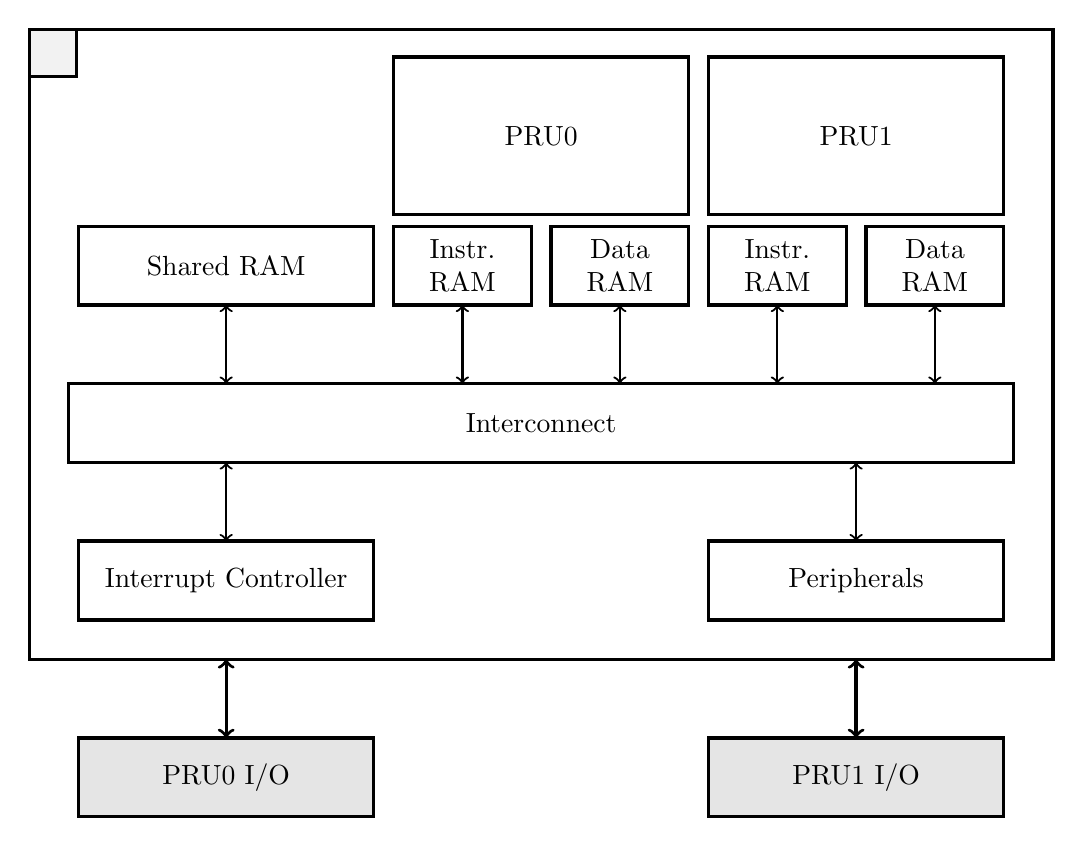
\begin{tikzpicture}[
			squarednode/.style={
				rectangle,
				draw=black,
				very thick,
				align=center,
				inner sep=0cm
			},
			main/.style={
				minimum width=13cm,
				minimum height=8cm
			},
			interconnect/.style={
				minimum width=12cm,
				text width=12cm,
				minimum height=1cm
			},
			sram/.style={
				minimum width=3.75cm,
				text width=3.75cm,
				minimum height=1cm
			},
			ram/.style={
				minimum width=1.75cm,
				text width=1.5cm,
				minimum height=1cm
			},
			pru/.style={
				minimum width=3.75cm,
				text width=3.5cm,
				minimum height=2cm
			}
		]

		\node[squarednode,main] (Box) at (0,1) {};
		\node[squarednode,below right,inner sep=3mm, fill = black!5] at (Box.north west) {\large\textbf{\pruss}};

		\node[squarednode,interconnect] (SharedRam) at (0,0) [] {Interconnect};

		\node[squarednode,sram] (IntC)  at (-4,-2) {Interrupt Controller};
		\node[squarednode,sram] (Peri)  at (4, -2) {Peripherals};

		\draw[thick, <->] (-4,-1.5) -- (-4,-0.5);
		\draw[thick, <->] (4, -1.5) -- (4, -0.5);

		\node[squarednode,sram, fill=black!10] (IntC)  at (-4,-4.5) {PRU0 I/O};
		\node[squarednode,sram, fill=black!10] (Peri)  at ( 4,-4.5) {PRU1 I/O};

		\draw[very thick, <->] (-4,-3) -- (-4,-4);
		\draw[very thick, <->] ( 4,-3) -- ( 4,-4);

		\node[squarednode,sram] (IntCon)  at (-4,2) {Shared RAM};
		\node[squarednode,ram] (Pru0IRAM) at (-1,2) {Instr. RAM};
		\node[squarednode,ram] (Pru0DRAM) at (1, 2) {Data RAM};
		\node[squarednode,ram] (Pru1IRAM) at (3, 2) {Instr. RAM};
		\node[squarednode,ram] (Pru1DRAM) at (5, 2) {Data RAM};

		\draw[thick, <->] (-4,1.5) -- (-4,0.5);
		\draw[thick, <->] (-1,1.5) -- (-1,0.5);
		\draw[thick, <->] (1, 1.5) -- (1, 0.5);
		\draw[thick, <->] (3, 1.5) -- (3, 0.5);
		\draw[thick, <->] (5, 1.5) -- (5, 0.5);

		\node[squarednode,pru] (PRU0) at (0, 3.65) {PRU0};
		\node[squarednode,pru] (PRU1) at (4, 3.65) {PRU1};

	\end{tikzpicture}
	\caption{Block diagram of the \pruss}
	\label{fig:pruss_block}
\end{figure}

 Because of this approach, every instruction takes \SI{5}{\nano\second}, and there is no pipelining, or out-of-order execution.

\subsection{Determinism of the \pru}

Texas Instruments' main goal with this coprocessor was to maximize the determinism of the processor, and the code running on it. This approach utilizes some unique design decisions.

\subsubsection{Execution}

On the \pru, every instruction takes \SI{5}{\nano\second} to execute. This is an interesting design pattern, because on most architecture the execution cycle varies with instructions e.g. the \emph{JUMP} instruction always need more execution cycle than a simple addition. The \pru aarchitecture is uniformial. This uniformity helps the static analysis of code, because there are no corner cases in the cycle counts.

There is no pipelining, and out-of-order execution, so the processor execute the machine code in the exact same order it was compiled.

\subsubsection{Interrupt handling}

There is no interrupt vector though the \pruss have an interrupt controller. The handling of interrupts is not hardware based like in other microcontrollers like the Microchip's PIC or the Atmel's AVR microcontrollers.

The default approach in interrupt handling is to interrupt the normal code execution, save the state of the normal execution (current program counter, and register values), and jump to an interrupt service routine (\textls{ISR}). After the ISR returns, the normal execution is restored, and continued.

On the \pru, there is no hardware based approach, the executed code must poll a specific register containing the flag bits of interrupt signals. By this way, the determinism of interrupt handling (despite the name \emph{interrupt} implies the interruption of normal execution flow) is fully handled by the executed code thus giving full control when these signals are processed.
